\section{Physical Experiments}

% \begin{figure}[t]
%     \centering
%     {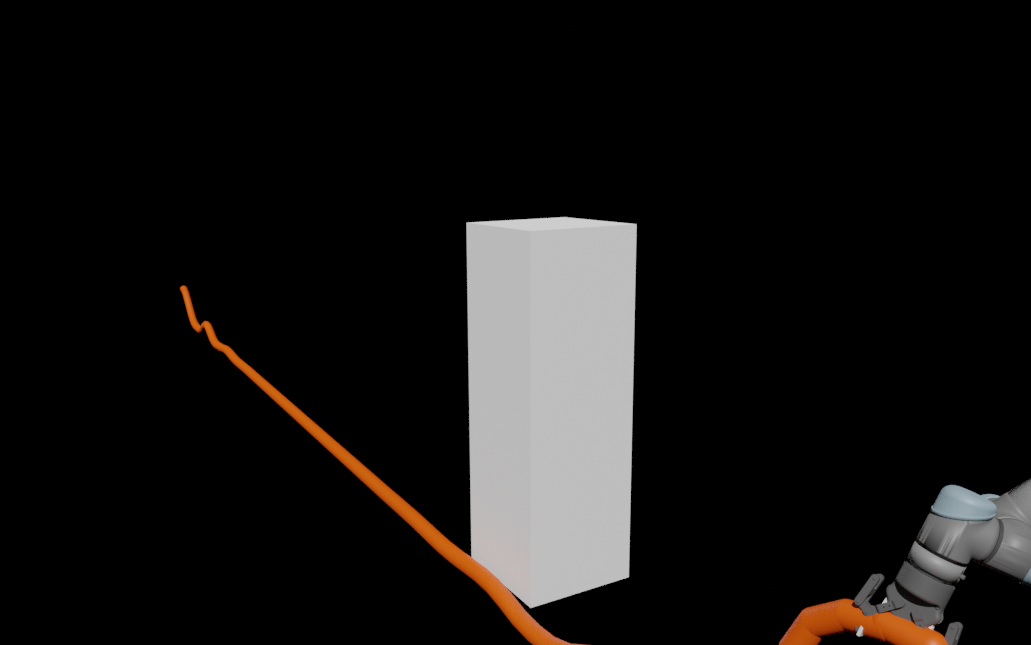
\includegraphics[width=.23\textwidth]{figures/sim_start.png}}\hfill
%     {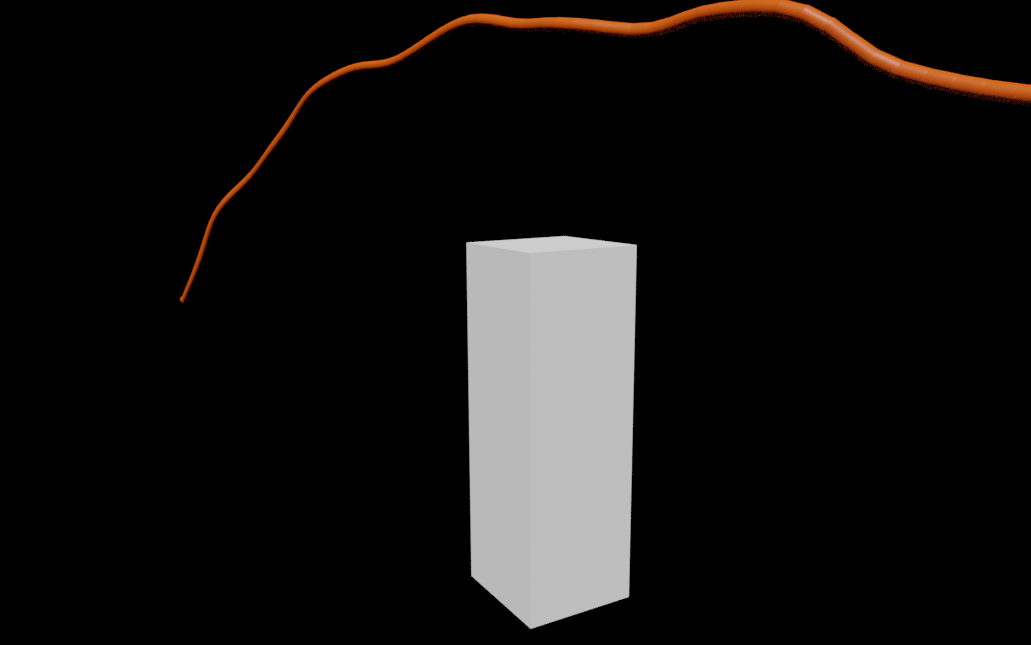
\includegraphics[width=.23\textwidth]{figures/sim_apex.png}}\hfill
%     {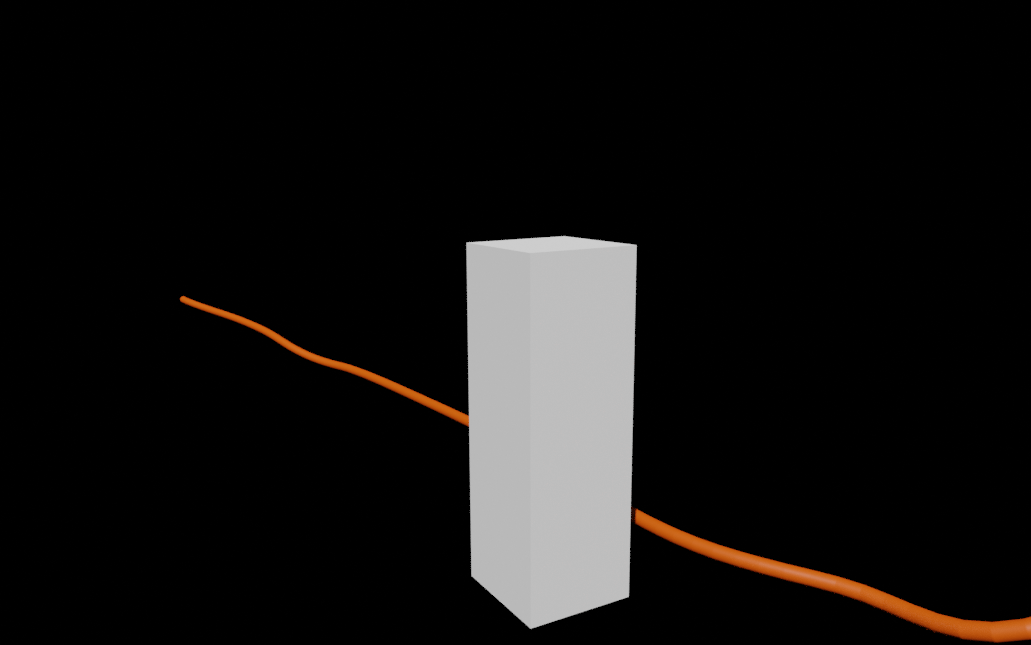
\includegraphics[width=.23\textwidth]{figures/sim_end.png}}
%     \caption{Cable trajectory for data generation in simulation (above) vs. cable trajectory in real (below) for the vaulting task.}
%     \vspace*{-10pt}
%     \label{fig:sim_to_real}
% \end{figure}
\begin{figure}
    \vspace*{5pt}
    \centering
    \begin{tabular}{@{}c@{\hspace{2.4pt}}c@{\hspace{2.4pt}}c@{}}
        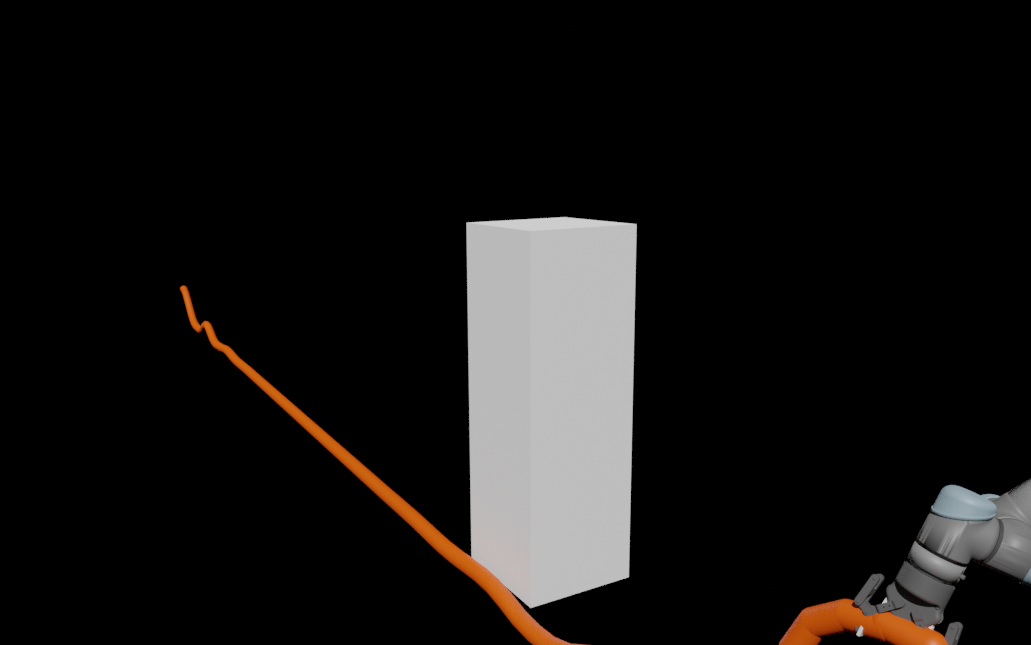
\includegraphics[width=80pt]{figures/sim_start.png} & 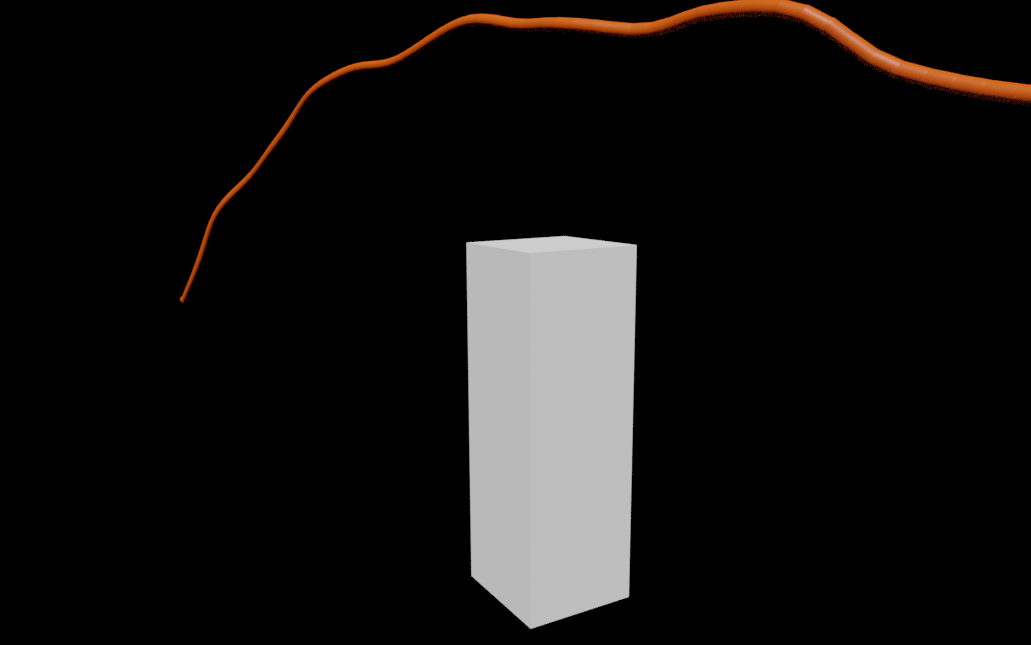
\includegraphics[width=80pt]{figures/sim_apex.png} & 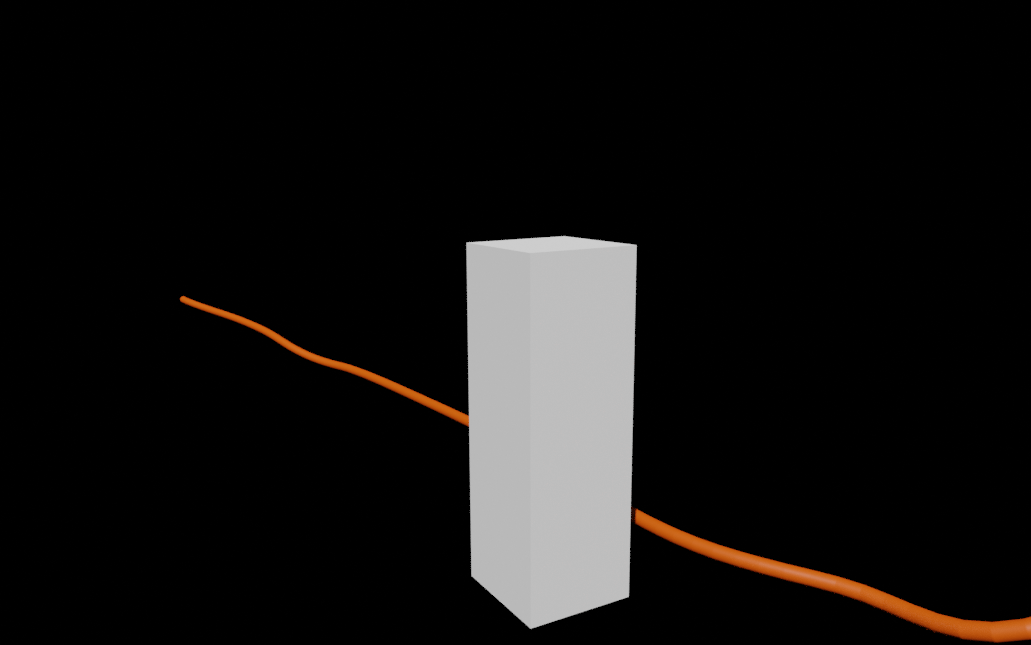
\includegraphics[width=80pt]{figures/sim_end.png} \\
        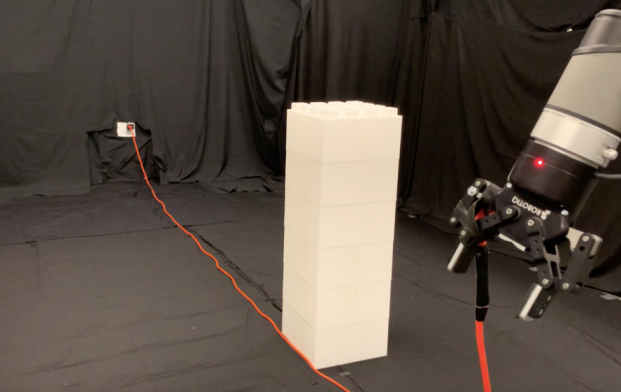
\includegraphics[width=80pt]{figures/real_end.png} & 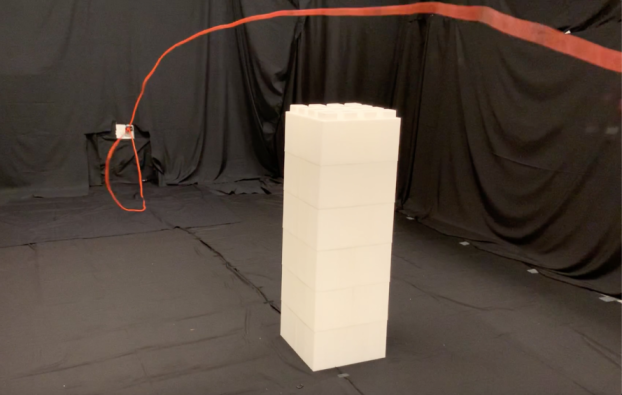
\includegraphics[width=80pt]{figures/real_apex.png} & 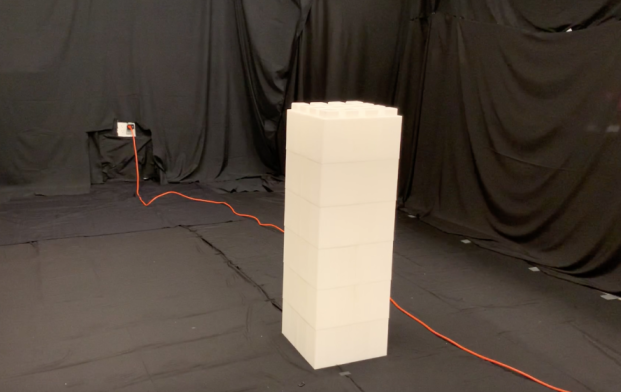
\includegraphics[width=80pt]{figures/real_start.png}\\
        \small{Start configuration} & \small{Apex configuration} & \small{End configuration}
    \end{tabular}
    \caption{Cable trajectory for data collection in \textbf{simulation (top)} vs. cable trajectory in \textbf{real (bottom)} for the vaulting task after applying the same apex point configuration.}
    \label{fig:sim_to_real}
    \vspace*{-10pt}
\end{figure}
\begin{figure}[t]
    \vspace*{5pt}
    \centering
    % \begin{tabular}{c@{\hspace{1.5pt}}c@{\hspace{1.5pt}}}
    %\subfloat[Trajectories defined by 3 points \label{fig:3point}]{%
      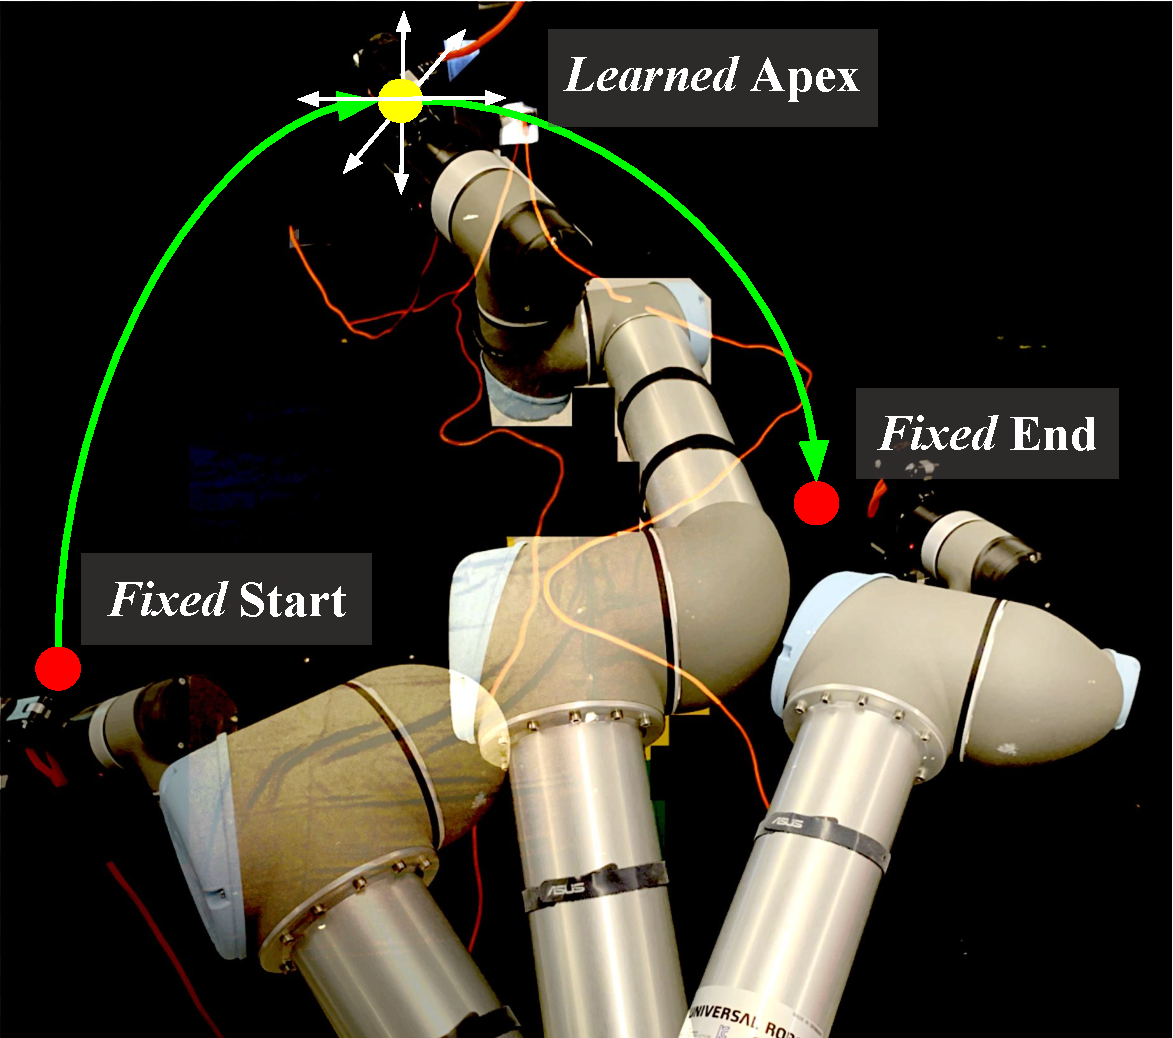
\includegraphics[height=110pt]{figures/3point.pdf}%}%
      \hfill
    %\subfloat[Physical space layout\label{fig:layout}]{%
      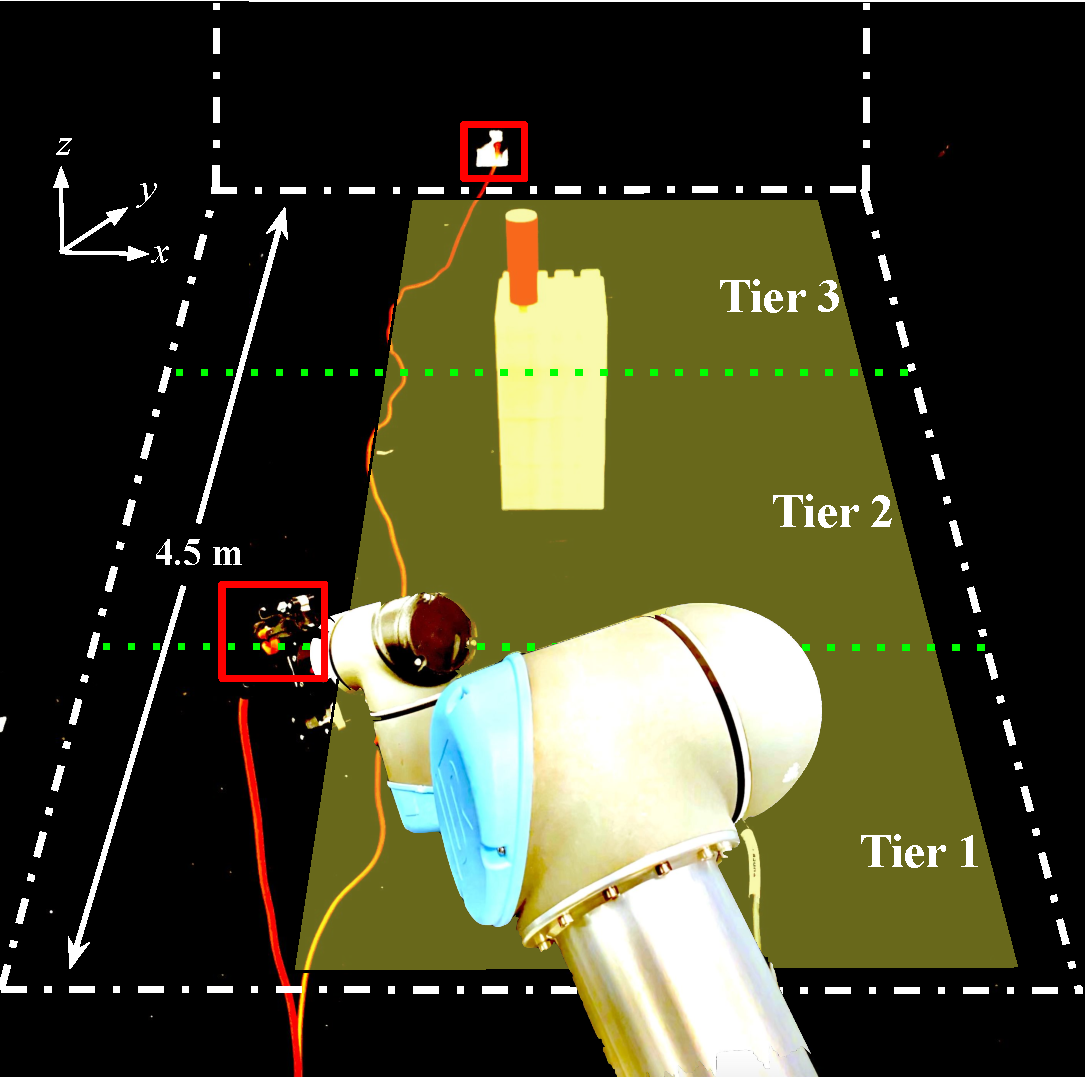
\includegraphics[height=110pt]{figures/layout_new.pdf}%}
    % \end{tabular}
    \caption{\textbf{Left: }Using three points in a curve to control the trajectory of the cable. The start and end points are fixed using the arm configurations. We change the trajectory by varying the apex configuration. \textbf{Right: }Design of physical experiments. We randomize the white Lego bricks’ location within the yellow shaded area. For vaulting and knocking, the width of the yellow area is 1.5~m, and 1.0~m for weaving. The yellow area is divided into three difficulty tiers.}
   % {\color{red} We need to change the label on the mid point.  Can you add arrows indicating that the mid point can by varied left/right and up/down (and in/out).  Also can you reverse the colors so that it starts/stops on red, and we vary the midpoint yellow.}}
    %    \vspace*{-10pt}
    \label{fig:motion_and_floor}
    \vspace*{-10pt}
\end{figure}

We use a physical UR5 robot grasping to dynamically manipulate a cable attached to a wall 4.5\,m away, on the three tasks, with 5 different cable types.
The system obtains observations from a Logitech C270 720p webcam placed 0.75\,m above the robot arm base.  It scales and crops the image to a 512x512x3 segmented RGB image that feeds into a ResNet-34~\cite{resnets_2016} deep neural network implemented with PyTorch~\cite{pytorch_neurips}.
We initialize weights using He initialization~\cite{he2015delving}.

%We use a UR5 arm on a fixed base because the arm can move fast enough to induce motions on the cable, and the fixed base allows us to control the experimental setup.
%The UR5's joints are specified to move up to 3\,rad/s, which we set as velocity constraints in the trajectory function.%, and observed the robot achieving.



%We attempted experiments on a Fetch~\cite{fetch}, but while its specification state the joints have limits in the range 1.52 to 2.27~rad/s, we found that its arm could not move quick enough to induce a similar motion on the cable.  We speculate that this may be a problem specific to the Fetch we attempted to use in our experiments.

%while the Fetch \harry{TODO: Find Fetch details.}

% \subsection{Simulation Environment}
% \jonathan{TODO: move to IV-D}
% In simulation, we compare the model that only regresses on the apex point with a model that outputs the velocity of the arm along with the apex point in the motion defined by the three points. To vary velocity of the arm in simulation, we modify the keyframe at which the arm reaches the apex point. For example, reducing the keyframe value would cause the arm to move from the start configuration to the apex point more quickly, and move from the apex point to the end configuration at a slower speed. Simulation allows for fair comparisons between our hypothesized models, as perfect resets could be done when comparing the velocity regression model to the apex point model. For simulated vaulting on randomized obstacle locations, the model that regresses both apex point location and velocity achieves a 70\% success rate, while the model that only regresses apex point location achieved a 76\% success rate. Furthermore, 27\% of the failure cases for the velocity regression model are successfully completed by the three-point model in the same setting, suggesting that simpler input is more reliable.


% \subsection{Real World Environment}
In physical experiments of the 3 tasks (see Fig.~\ref{fig:motion_and_floor} for layout),
% \begin{figure}[t]
    \centering
    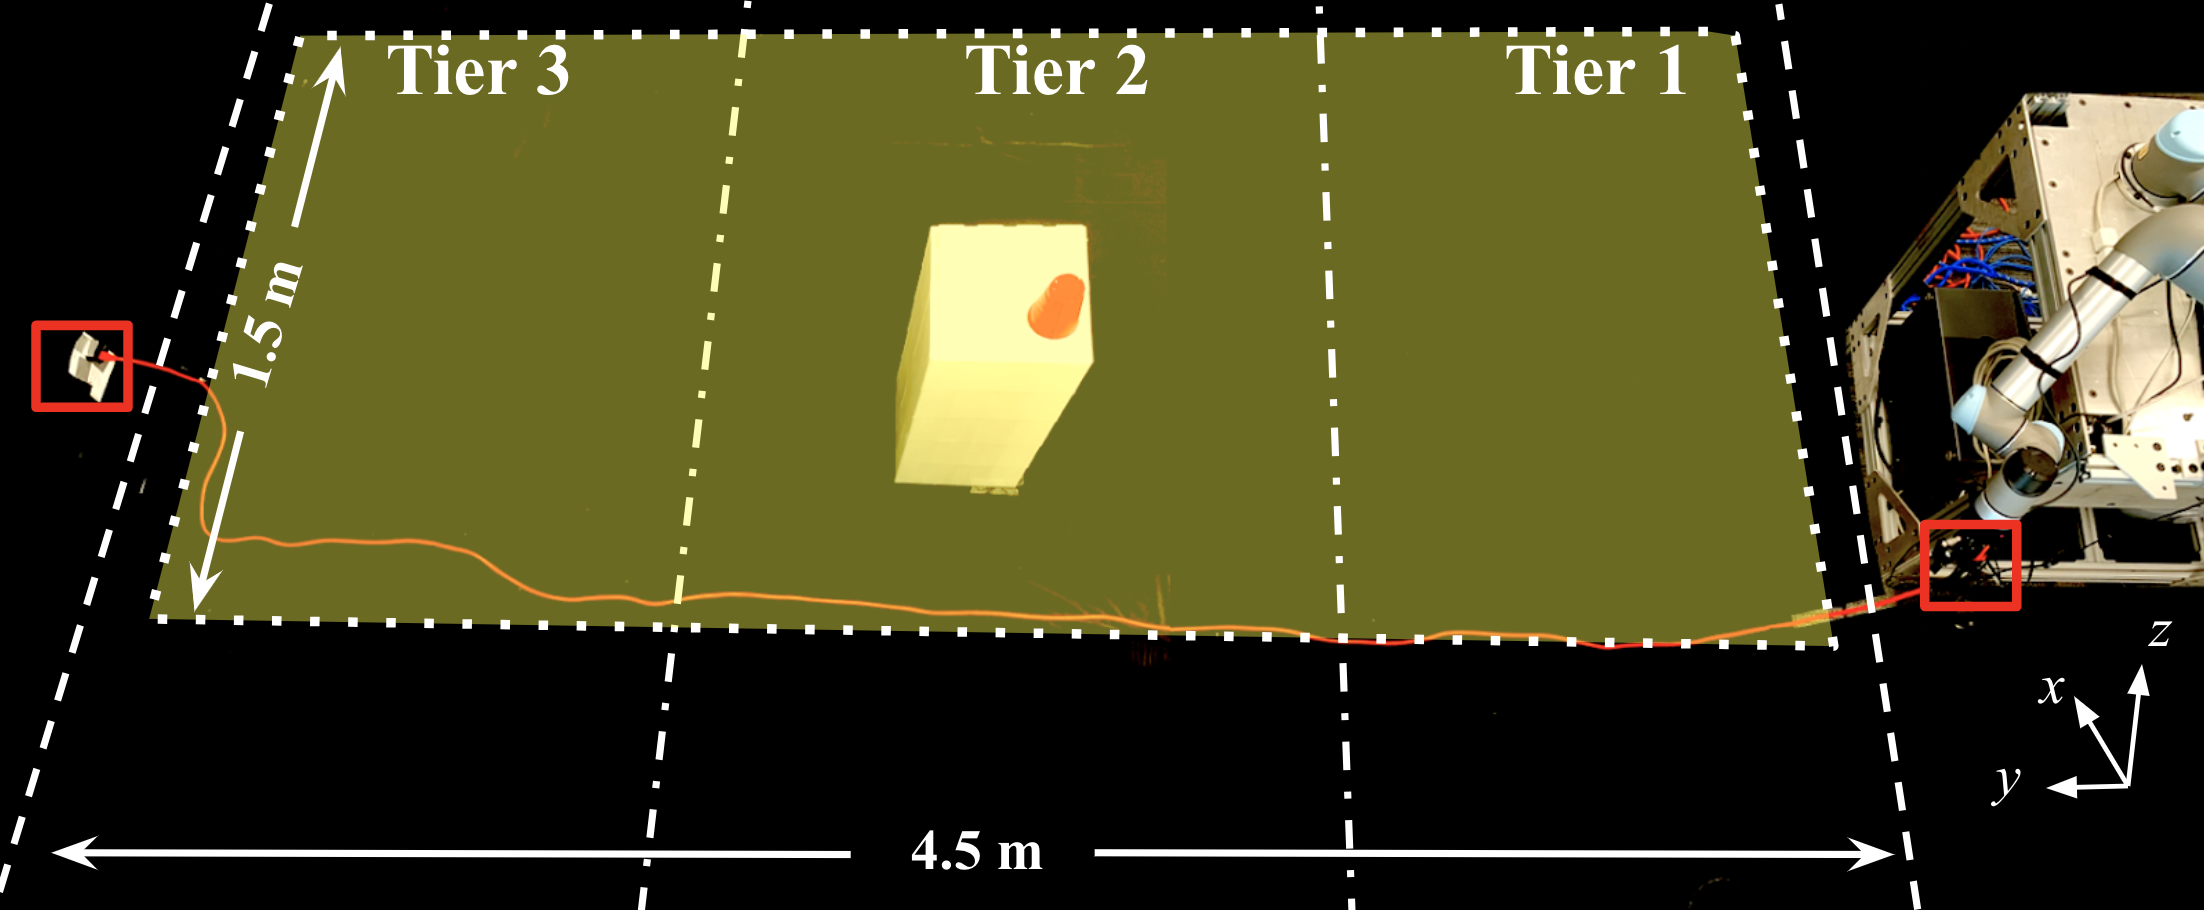
\includegraphics[width=\linewidth]{figures/layout.png}
    \caption{Design of physical experiments. We randomize the white Lego bricks' location within the yellow shaded area for vaulting and knocking. The yellow shaded area is also broken down into three difficulty tiers. Here we show an example of knocking, where the white Lego bricks form a base for the red target object on top of it and the robot aims to knock over the red target. \harry{TODO: prof. G said rotate. need to find a better way to convey the idea.}}
    \vspace*{-10pt}
    \label{fig:layout}
\end{figure}
we use large, white plastic bricks as the obstacle(s), which can vary in size and location. The obstacles we use for experiments are 0.15\,m to 0.75\,m in width and 0.3\,m to 1.5\,m in height.
To generate training data, we randomize the location and size of the obstacles in each trial.
We test the system with 5 cables listed in Table~\ref{tab:cable_types}.
%We test our system with 4 different types of cables of different lengths and calibers: a 5.5-meter orange 18-gauge power extension cable, a 5-meter white 16-gauge power extension cable, a 6.2-meter orange 14-gauge power extension cable, and a 5.5-meter blue 22-gauge ethernet cable. We also test our system on a 4.8-meter blue 12-gauge jump cable. The UR5 station's base is 4.5 meters away from the fixed end of the cable.

\begin{table}[t]
    \vspace*{4pt}
    \centering
    \caption{Physical cables used in experiments and the number of successes in the three tasks (Vaulting, Knocking, Weaving) using policies trained with the 18 AWG orange cable. For each cable, we evaluate with 20 trials for each task.}
    \begin{tabular}{@{}l@{\quad}r@{\quad}r@{\quad}r@{\quad}r@{\quad}r@{}}\toprule
        
         Type & kg & m & Vaulting & Knocking & Weaving \\
        \midrule
         18 AWG orange cable  & 0.65 & 5.5 & 16&13&12\\
         16 AWG white cable   & 0.70 & 5.2 &16&12&12\\
         16 AWG orange cable  & 0.90 & 6.2 &4&2&2\\
         22 AWG blue network cable  & 0.48 & 5.5 &14&9&12\\
         12 AWG blue jump rope   & 0.45 & 5.1 &15&10&8\\
         %5-meter white 16-gauge power extension cable, a 6.2-meter orange 14-gauge power extension cable, and a 5.5-meter blue 22-gauge ethernet cable. We also test our system on a 4.8-meter blue 12-gauge jump rope. 
         \bottomrule
    \end{tabular}
    \vspace*{-16pt}
    \label{tab:cable_types}
\end{table}

%With the starting, apex, and ending joint configurations of the robot, we feed them into the QP solver to solve for a fast, min-jerk trajectory. Once the robot executes this trajectory, we check if the trial succeeds and record data accordingly.%, where we only record the 3 joint angles of the robot at the apex of the motion when the resulting trajectory succeeds.

We define \emph{difficulty tiers} based on the distance of the obstacle to the base of the robot.
% \begin{tabular}{@{}l|l|l@{}}
%     \textbf{Tier 1: ${\pmb{\leq}}$ 1.5\,m} & 
%     \textbf{Tier 2: 1.5 to 3\,m} & 
%     \textbf{Tier 3: ${\pmb{\geq} }$ 3\,m}
% \end{tabular}
%
\begin{table}[h]
\centering
\vspace{-6pt}
\begin{tabular}{@{}ccc@{}}
    \textbf{Tier 1} & 
    \textbf{Tier 2} & 
    \textbf{Tier 3} \\
    ${\pmb{\leq}}$ 1.5\,m &
    1.5 to 3\,m & 
    ${\pmb{\geq} }$ 3\,m
\end{tabular}
\vspace{-12pt}
\end{table}
%
%
% \begin{description}
%     \item \textbf{Tier 1: ${\pmb{\leq}}$ 1.5~m} 
%     % The objects of interest are less than 1.5 meters away from the base of the robot.
%     \item \textbf{Tier 2: 1.5 to 3~m} 
%     % The objects of interest are 1.5 to 3 meters away from the base of the robot.
%     \item \textbf{Tier 3: ${\pmb{\geq} }$ 3~m} 
%     % The objects of interest are more than 3 meters away from the base of the robot.
% \end{description}
%

We evaluate INDy along with two baselines:
%
\begin{description}[align=left,leftmargin=0pt]
    \item[Baseline with Fixed Apex.] In the three tasks, for each configuration, a human annotator sets one set of apex joint angles that can accomplish the task. The apex joint angles are fixed with respect to the obstacle itself, and they remain the same across different locations of the same obstacle.
    \item[Baseline with Varying Apex.] In vaulting and weaving, for each configuration (including obstacle size and location), a human annotator sets the apex joint angles such that the robot arm's end effector is 15\,cm above the center of mass (COM) of the obstacle, and aligned horizontally with the COM of the obstacle. For knocking, a human annotator makes the robot arm end 10\,cm above the COM of the target object, and aligned horizontally with the COM.
\end{description}

We find the baselines from simulation, where we observe that the fixed and varying apex motions could induce enough velocity to make the cable vault the obstacle.